%!TEX root = ../BGP_for_networks_who_peer.tex
\chapter{iBGP - BGP within one Autonomous System}
\section{What is iBGP?}
iBGP is not a separate protocol. It is simply the ``flavor'' of BGP which is spoken between routers which are in the same \glsreset{AS}\gls{AS}.

All BGP routers use \gls{TCP} to communicate with each other.

Prefixes are distributed in iBGP according to the following rules:
\begin{itemize}
  \item Each router only distributes the best route for a prefix
  \item Prefixes received via iBGP (from the same \gls{AS}) are \emph{not} distributed
  \item Prefixes received via eBGP (from other \glspl{AS}) are distributed.
\end{itemize}
Since prefixes received from routers via iBGP are not redistributed (there are exceptions, see \ref{routereflector}), iBGP has to be \emph{fully meshed}, meaning that each router needs to have an iBGP session to all other routers.

By default, the next-hop address of a prefix received via eBGP is redistributed \emph{unchanged}. If you do not want to redistribute the IP addresses (IPv4 and IPv6) of external interfaces within your \gls{AS}, you need to set an option on your iBGP sessions to change this next-hop address to the address of your iBGP session. Usually this option is named \emph{next-hop-self}.

BGP4 is multi-protocol capable. That means that you can use IPv4 to both distribute IPv4 and IPv6 prefixes. However, this is not really advisable, as the next-hop address (which is also distributed) has to be set manually then. Best practice is to use IPv4 transport to distribute IPv4 prefixes and IPv6 transport to distribute IPv6 prefixes.

\section{Configuring iBGP}
Like stated above, iBGP uses \gls{TCP} to communicate. So to set up an iBGP session between two routers, you need to define:
\begin{itemize}
  \item IP address to connect to
  \item local IP address to be used as source (optional, but recommended)
\end{itemize}

\subsection{About the Loopback interface}
If you do not tell BGP which local IP address to use, routers use as source IP the IP address of that interface on which packets leave the router. This might not be advisable, because if that interface goes down all iBGP sessions using the IP address of this interface get disrupted, even if there is another path to the remote router.

\begin{figure}
  \centering
  \includegraphics[width=\linewidth,page=11]{img/Drawings.pdf}
  \caption{iBGP connection with and without Loopback interface}
  \label{fig:ibgploopback}
\end{figure}

Therefore, best practice is to define a \emph{Loopback interface}, an artificial internal interface which is not connected to anything and always stays up. As the Loopback interface is not connected to anything, the address of the Loopback interface should be a /32 in IPv4 and a /128 in IPv6.

This is illustrated in figure \ref{fig:ibgploopback} - if an interface IP is used, the TCP connection gets disrupted in the instance of a circuit failure and has to be re-established (of course the iBGP connection also has to be re-established, including the exchange of all BGP prefix information). If a Loopback interface is used, the TCP connection is simply re-routed and the iBGP connection will stay up.

Also, for IPv6 you can easily use link-local addresses on the interconnect and just have the Loopback statically configured and use it for iBGP. If you have the luxury to choose, you might have ``similar looking'' IPv4 and IPv6 addresses for the Loopback interface. But beware of giving your IPv6 addresses any ``meaning'' - just select an IPv6 prefix and assign addresses out of it. Otherwise, you will run into problems later on, as giving meaning to addresses seldom scales.

\subsection{Lifecycle of a BGP connection}
If you configure BGP on a router, if the session comes up, everything is fine. But sometimes the session cannot be established, and if you check the BGP session table you might see a ``status'' of the session. Some of these states that a session can be in are self-explanatory, but some require more explanation. You will find below a list of session states you might see. These session states are defined in \rfc{4271} as a finite state machine. All states described are \emph{per peer}.

\begin{figure}
  \centering
  \includegraphics[width=\linewidth,page=15]{img/Drawings.pdf}
  \caption{BGP finite state machine}
  \label{fig:bgpfsm}
\end{figure}

\begin{description}
  \item[Idle] is the initial state of any BGP connection. In this state, no resources are allocated to the session and incoming connection attempts are refused. Depending on events, the state is either changed to \emph{active} or \emph{connect}.
  \item[Connect] means that BGP is waiting for a TCP connection to a neighbor to be completed. If this succeeds, the state of the session is changed to \emph{OpenSent}, if not, it's either back to \emph{idle} or to \emph{active}.
  \item[Active] - you will see this state a lot. Be aware that it means that a BGP session is \emph{not} established. BGP in this state waits for an incoming TCP connection. If the retry timer expires, the state changes to \emph{connect} to re-try connecting.
  \item[OpenSent] - BGP has established a TCP connection, sent an \emph{open} message to the peer and waits for an incoming \emph{open} message. Once received and checked ok, the state is changed to \emph{OpenConfirm}. In case of a timeout or an error, the state falls back to either \emph{idle} or \emph{active}.
  \item[OpenConfirm] - here BGP waits for a \emph{keepalive} or \emph{notification} message from the peer. We are nearly there! If one of these messages are received, the state is changed to \emph{established}. If something goes wrong, again we fall back to either \emph{idle} or \emph{active}.
  \item[Established] is the state that you want your BGP session to be in. Prefixes can be exchanged and everything is fine. From here you can only go back to \emph{idle}.
\end{description}
See also figure \ref{fig:bgpfsm} for the states and how they may change.

\subsubsection{Notifications on shutdown}
When a BGP session is shut down, the party initiating the cease of the BGP session is sending out a notification. \rfc{4486} lists a number of pre-defined reasons for shutting down a session.
\begin{description}
  \item[Maximum number of prefixes reached] - this means that the other side is sending more prefixes then the receiver allows (see \ref{maxprefix}). Sending of this notification is mandatory.
  \item[Administrative shutdown] - the session has been shut down using a configuration command.
  \item[Peer de-configured] -  the BGP session has been de-configured.
  \item[Administrative reset] - the session has been reset using a command. It will be re-established again.
  \item[Connection rejected] - if the BGP session is disallowed \emph{after} a TCP session has already been established this notification should be sent.
  \item[Other configuration change] - if a session is reset for any other reason as the ones stated above.
  \item[Connection collision resolution] - this should be sent if a collision occurs  while establishing a session.
  \item[Out of resources] - this may be sent if a router runs out of resources (like memory) and tears down the session.
\end{description}

The newer \rfc{8203} enhances the \emph{Administrative Reset} and \emph{Administrative Shutdown} reasons with the possibility for the shutting down party to add a free-form text message.

It is up to the receiver of all these notifications to do something with them (or not) - for example the DE-CIX route server displays them in the looking glass - see \url{https://lg.de-cix.net}.

\subsubsection{Timers}
To keep BGP sessions alive (well, more to check \emph{if} they are still alive) BGP speakers send each other \emph{keepalive} messages. The following timers  exist:
\begin{description}
  \item[Keepalive Timer:] This timer takes care of sending \emph{keepalive} messages to the BGP neighbor. Everytime it expires a keepalive message is sent and the timer is reset (it is also reset every time a normal update message is sent). The start value of the Keepalive Timer may be configurable, it is usually one third of the Hold Timer.
  \item[Hold Timer:] This timer determines how long a BGP session is considered being open without a \emph{keepalive} or update message received. The start value of the timer is negotiated during session setup - it is usually three times of the initial value of the \emph{Keepalive Timer}. It can be configured on a per-neighbor basis and in session initiation the lowest value configured of the two peers wins. A usual default value is 180 seconds. It is not a good idea to set this timer too aggressively short - this would increase the CPU load of the BGP process.

  If the hold timer expires, the BGP session is considered being down and all prefixes received from this session are removed from the BGP table and the session state is set to \emph{idle}.
\end{description}

Given the usual default values it may take up to three minutes to detect if a BGP neighbor is down. During that time, if the interface the session is established on is still up, prefixes received via this session are still valid and so traffic may be dropped.

% For a faster detection if a neighbor is down today usually \gls{BFD} is used.

\fcolorbox{black}{lgray}{
\begin{minipage}{\linewidth}
\dangersign[8ex] \textbf{Recommendation:}
Do not modify the BGP timers unless you are absolutely sure you know what you are doing. If you want to take down BGP sessions fast if a neighbor goes down, use \gls{BFD}
\end{minipage}
}



\subsection{Fully Meshed vs. Route Reflector}
\label{routereflector}
As an iBGP speaker by default does not forward prefixes received via iBGP, your iBGP nodes need to be \emph{fully meshed}. This means each BGP speaking router needs an iBGP connection to any other BGP speaking router (with $n$ routers, each router therefore has $(n-1)$ iBGP sessions; in your network you have $n*(n-1)/2$ iBGP sessions in total).

\begin{figure}
  \centering
  \includegraphics[width=\linewidth,page=12]{img/Drawings.pdf}
  \caption{Application of a Route Reflector}
  \label{fig:routereflector}
\end{figure}

Now imagine one of your edge routers is connected in a non-redundant way to the rest of your network (see figure \ref{fig:routereflector}). There is no point setting up multiple iBGP sessions - if the connection to this edge router fails, \emph{all} of them will go down. This is a good application for using a \emph{Route Reflector}. A \gls{Route Reflector} sends out all prefixes (even those received via iBGP) to its \glspl{Route Reflector Client}. These clients usually have only one BGP connection - to their server.

Using route reflection, it is also possible to build iBGP networks using only Route Reflectors and clients. These architectures are beyond the scope of this document.

Configuration has only to be done on the reflector side; usually it's just one statement.
\begin{description}
  \item[Cisco:] \begin{verbatim}
    neighbor 172.16.1.2 route-reflector-client
    neighbor 172.16.1.2 next-hop-self all
\end{verbatim}
  ``next-hop-self all'' sets the next hop of announced prefixes to the IP of the reflector for all prefixes announced to the client. With this set, you might not even have to run an \gls{IGP} on your client.
  \item[Mikrotik:] \begin{verbatim}
  /routing bgp peer
  add name=R2 nexthop-choice=force-self \
    remote-address=172.16.1.2 \
    remote-as=64500 route-reflect=yes
\end{verbatim}
The ``force-self'' in nexthop-choice sets the interface IP of the reflector as nexthop when announcing prefixes to the client.
  \item[Juniper:] To configure a route reflector you simply have to give it a \emph{cluster} id, best is to do that in a group: \begin{verbatim}
  protocols {
      bgp {
          local-as 64500;
          group internal-rr {
              type internal;
              family inet {
                  unicast;
              }
              export rr-next-hop;
              cluster 172.16.1.1;
              peer-as 64500;
              neighbor 172.16.1.2;
          }
      }
  }
\end{verbatim}
Setting the next hop is done with a policy-statement: \begin{verbatim}
policy-options {
  policy-statement rr-next-hop {
      term 1 {
          from protocol bgp;
          then {
              next-hop self;
          }
      }
  }
}
\end{verbatim}
\end{description}

In this case, using a Loopback interface for the session and for next-hop is not advisable. The client is not connected redundantly, so if the connection goes down a Loopback interface does not help. Also, when using the interface IP for the iBGP session \emph{and} a forced next-hop for announced prefixes, you do not even have to run an \gls{IGP} to the client.

\subsection{Keeping the configuration short}
In general, it is advisable to keep the iBGP configuration as short as possible. Depending on the router you are using, there is the possibility to group BGP commands. On Cisco this is called a ``peer group''.

To keep IPv4 and IPv6 configuration separate, use one peer group for each - also most routers do not allow mixing of configuration here.

\subsection{Cisco example}
Configuration example for Loopback interface and iBGP for Cisco IOS:
\begin{verbatim}
  interface Loopback0
    ip address 172.16.1.1 255.255.255.255
    ipv6 address 2001:db8:500::1:1/128
  !
  router bgp 64500
    neighbor internal peer-group
    neighbor internal remote-as 64500
    neighbor internal update-source Loopback0
    !
    neighbor internal6 peer-group
    neighbor internal6 remote-as 64500
    neighbor internal6 update-source Loopback0
    !
    neighbor 172.16.1.2 peer-group internal
    neighbor 172.16.1.3 peer-group internal
    neighbor 172.16.1.4 peer-group internal
    !
    neighbor 2001:db8:500::1:2 peer-group internal6
    neighbor 2001:db8:500::1:3 peer-group internal6
    neighbor 2001:db8:500::1:4 peer-group internal6
    !
    address-family ipv4
      neighbor internal next-hop-self
    !
    address-family ipv6
      neighbor internal6 next-hop-self
    ...
\end{verbatim}
This is the minimum configuration. The local AS number is specified in the router command and the remote AS in the peer group.

The ``next-hop-self'' command ensures that prefixes received from other ASes  get this router's IP set as next-hop address (so external IPs do not have to be redistributed using our IGP). Note that this is below the ``address-family'' statement.

To set up iBGP sessions to each remote router, you need only configure its IP address and that it belongs to the peer group ``internal''.

To distribute the IP address of the Loopback interface, we extend the configuration of our IGP as shown in \ref{example-ospf}:
\begin{verbatim}
  router ospf 64500
    network 192.168.2.0 0.0.0.255 area 0
    redistribute connected subnets
\end{verbatim}
So again: We set up iBGP sessions between the Loopback interfaces of all routers.

For IPv6, if you use IS-IS, simply enable it on the Loopback interface:
\begin{verbatim}
  interface Loopback0
    ip router isis
    ipv6 router isis
\end{verbatim}

Similarly for OSPFv3; here you also have to add the number of the OSPFv3 process and an area:
\begin{verbatim}
  interface Loopback0
    ipv6 ospf 64500 area 0
\end{verbatim}

\subsection{Mikrotik example}
Mikrotik does not directly support Loopback interfaces, but you can use an empty bridge interface instead:
\begin{verbatim}
  /interface bridge
  add name=loopback0
  /ip address
  add address=172.16.1.1/32 interface=loopback0 network=172.16.1.1
  /ipv6 address
  add address=2001:DB8:500::1:1/128 interface=loopback0
\end{verbatim}

As an \gls{IGP}, Mikrotik only supports OSPFV2 and OSPFv3:
\begin{verbatim}
  /routing ospf-v3 interface
  add area=backbone interface=loopback0
  add area=backbone interface=ether1
  add area=backbone interface=ether2
  ...
\end{verbatim}

Also, Mikrotik does not support peer groups; you have to configure everything in the peer entry:
\begin{verbatim}
  /routing bgp instance
  set default as=64500 router-id=172.16.1.1

  /routing bgp peer
  add name=R2 nexthop-choice=force-self remote-address=172.16.1.2 remote-as=\
    64500 update-source=loopback0
  add name=R3 nexthop-choice=force-self remote-address=172.16.1.3 remote-as=\
    64500 update-source=loopback0
  add name=R2-6 nexthop-choice=force-self remote-address=2001:db8:500::1:2 \
    remote-as=64500 address-families=ipv6
  add name=R3-6 nexthop-choice=force-self remote-address=2001:db8:500::1:3 \
    remote-as=64500 address-families=ipv6
\end{verbatim}

We restrict the IPv6 iBGP sessions to IPv6, using the ``address-families'' statement. Otherwise the IPv6 sessions would want to announce IPv4 prefixes as well, and we decided to keep this separate. On the IPv4 sessions, the address-families config is not required, as IPv4 is distributed by default.

Also keep in mind that on both sides of an iBGP (or any BGP) session, the same address families must be configured - otherwise the session does not come up.

% \subsection{Juniper Example}
